%DEFINITIONS FOR THE PAPER
\documentclass[a4paper, 11pt]{article}
\usepackage[utf8]{inputenc}
\usepackage[T1]{fontenc}
\usepackage[top=3.0cm, bottom=2.43cm, right=3.0cm, left=3.0cm]{geometry}
%\usepackage{fontspec} % include OTF fonts, requires XeTeX
%\defaultfontfeatures{Ligatures=TeX}
\usepackage{filecontents}
%\usepackage{natbib} % bibliography style
\usepackage[backend=bibtex]{biblatex}
%\setcitestyle{open={(},close={)}}
\usepackage{subfigure} % multiple figures in LaTeX
\usepackage{wrapfig}
%\usepackage{comment}
\usepackage{multirow} % multiplerows in tables
\setlength{\parindent}{0.25in}
\setlength{\parskip}{1.3em}
\renewcommand{\baselinestretch}{1.2}
\usepackage{titlesec}
\usepackage{booktabs} % Better horizontal rules in tables
\usepackage[all,defaultlines=3]{nowidow} % avoids widow and orphan sentences
\usepackage{amsmath} % good math formulas
\usepackage{relsize} % increase size of formulas
\usepackage{subfiles} % to handle multiple documents
%microtype package
\usepackage[activate={true,nocompatibility}, final, tracking=true,kerning=false,spacing=false]{microtype}
\usepackage{authblk}
\renewcommand\Authfont{\fontsize{11}{13}\selectfont}
\renewcommand\Affilfont{\fontsize{10}{12}\itshape}
\titleformat*{\section}{\large\bfseries}
\pagenumbering{gobble}% Remove page numbers (and reset to 1)

%END OF DEFINITIONS

% Paper title

\title{\bfseries Satellite image time series analysis with the sits package}
%no date
\date{\vspace{-5ex}}
\author[1]{\normalsize Gilberto Camara}
\author[2]{\normalsize Victor Maus}
\author[1]{\normalsize Luiz Fernando Assis}
\author[1]{\normalsize Rolf Simoes}
\author[1]{\normalsize Adeline Maciel}
\author[1]{\normalsize Gilberto Ribeiro de Queiroz}

\affil[1]{\small Image Processing Division, National Institute for Space Research (INPE), Av dos Astronautas 1758, Sao Jose dos Campos, 12227-001 Brazil. \break
	Email: \{gilberto.camara\}@inpe.br}
\affil[2]{\small International Institute for Applied System Analyis, Schlossplatz 2, 2631 Laxenburg, Austria}

\usepackage{Sweave}
\begin{document}
\Sconcordance{concordance:sits_intro.tex:sits_intro.Rnw:%
1 50 1 1 0 1 1 1 6 29 1}

\fontfamily{put}\selectfont % Utopia
\maketitle

%1. Introduction:
%2. Time Series for LUCC Classification
%3. Land
%4. A framework for data modelling on land use semantics


A satellite image time series is...

first, get information about the WTSS (web time series service)
see WTSS paper for more information ("Web Services for Big Data")
\begin{figure}
\begin{Schunk}
\begin{Sinput}
> library(sits)
> URL <- "http://www.dpi.inpe.br/tws/wtss"
> inpe <- sits_configWTSS (URL,
+                  coverage = "mod13q1_512",
+                  bands = c("ndvi", "evi", "nir"))
> long <- -55.51810
> lat <-  -11.63884
> series.tb <- sits_getdata(longitude = long, latitude = lat, wtss = inpe)
> series.tb %>%
+      sits_select (bands = "evi") %>%
+      sits_plot ()
\end{Sinput}
\end{Schunk}
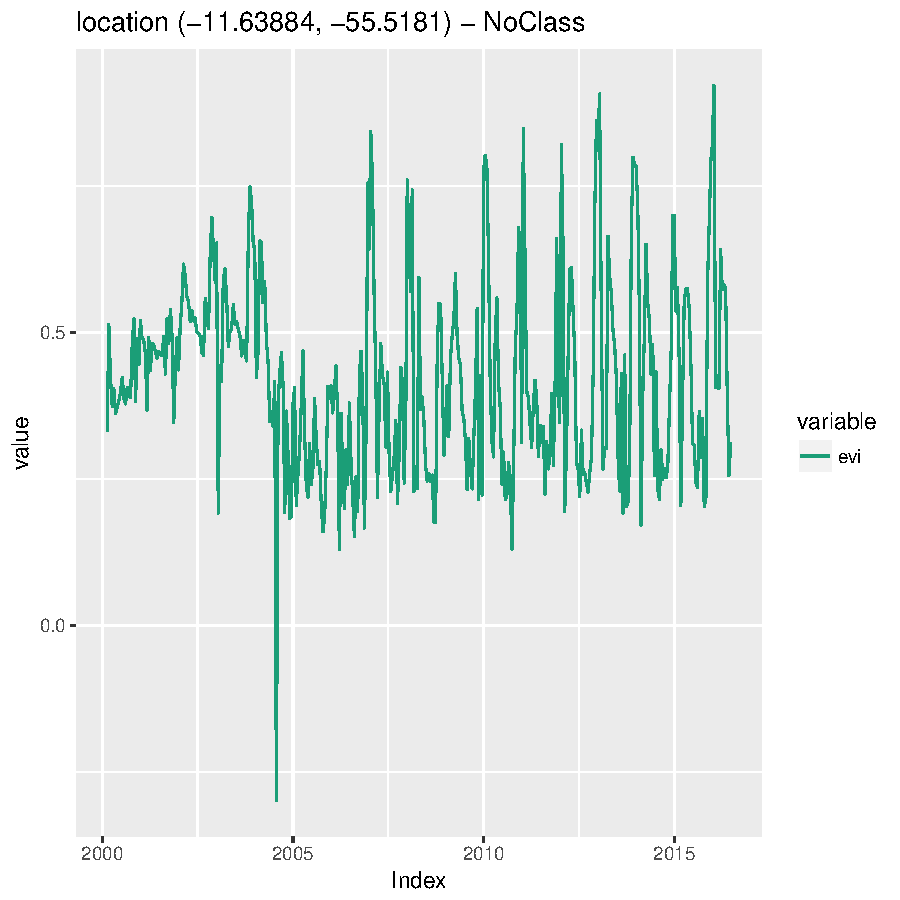
\includegraphics{sits_intro-001}
\caption{Time series for EVI band}
\end{figure}
which shows the time series for the "evi" band
%\input{introduction.Rnw}

\section{Introduction}
\label{sec:introduction}

%Stating the problem
Earth observation (EO) satellites produce vast amounts of geospatial data. The Landsat archive holds over five million images of the Earth's surface, with about 1 PB of data. New satellites from Europe, USA, China, Brazil, and India generate yearly as much data as one Landsat satellite in a decade. Most space agencies have adopted an open data policy, making unprecedented amounts of satellite data available for research and operational use. This data deluge has brought about a major challenge for Geoinformatics research: \textit{How to design and build technologies that allow the EO community to analyse big data sets?}

When scientists use big EO data they face the burden of organising thousands of files, downloaded from the space agencies archives. To manage such large data sets, researchers need stable and efficient solutions that support their analytical tasks. To choose a solution is hard because the technology for large data handling and analytics is evolving. Alternatives include MapReduce-based solutions such as Google Earth Engine \cite{Gorelick2012}, object-relational DBMS extensions such as Rasdaman \cite{Baumann1998} and  distributed multidimensional array databases such as SciDB \cite{Stonebraker2013}. Since each of these architectures takes on a different approach, understanding the benefits and drawbacks of each one helps researchers choose what best fits their needs.

Given the diversity of options, researchers would gain from documented experience that helps them to assess how proposed big data architectures fit the needs of geospatial data analysis. Recent papers describe algorithms required for EO analysis \cite{Vatsavai2012} \cite{Nativi2015} and report case studies using specific architectures \cite{Planthaber2012}\cite{Krcal2015}. However, to make progress on big geospatial data analysis, we need to engage the large community of remote sensing researchers. In this paper, we consider how big EO data architectures can support the needs of data analytics. Our paper examines ways to cut the effort required for researchers to develop and validate algorithms for extracting information for big EO data.

We take the viewpoint that architectures should serve applications, and not the other way around. To clarify the researcher's problem, we consider the needs for an important EO application: land use and land cover change (LUCC) analysis. We propose an architecture based on open-source tools that combines array databases with statistical analysis.  We evaluate this design to assess how it meets the needs of EO scientists and compared with other approaches that aim to meet these needs. This paper also puts forward a set of criteria to build researcher-friendly architectures for big EO data analysis.

%\bibliographystyle{abbv}
\bibliography{references-esensing.bib}
\end{document}
